% Appendix A

\chapter{Figuras adicionales}
\label{apendiceA}
\lhead{Apéndice B. \emph{Figuras adicionales}}

\begin{landscape}
\begin{figure}[h]
\centering
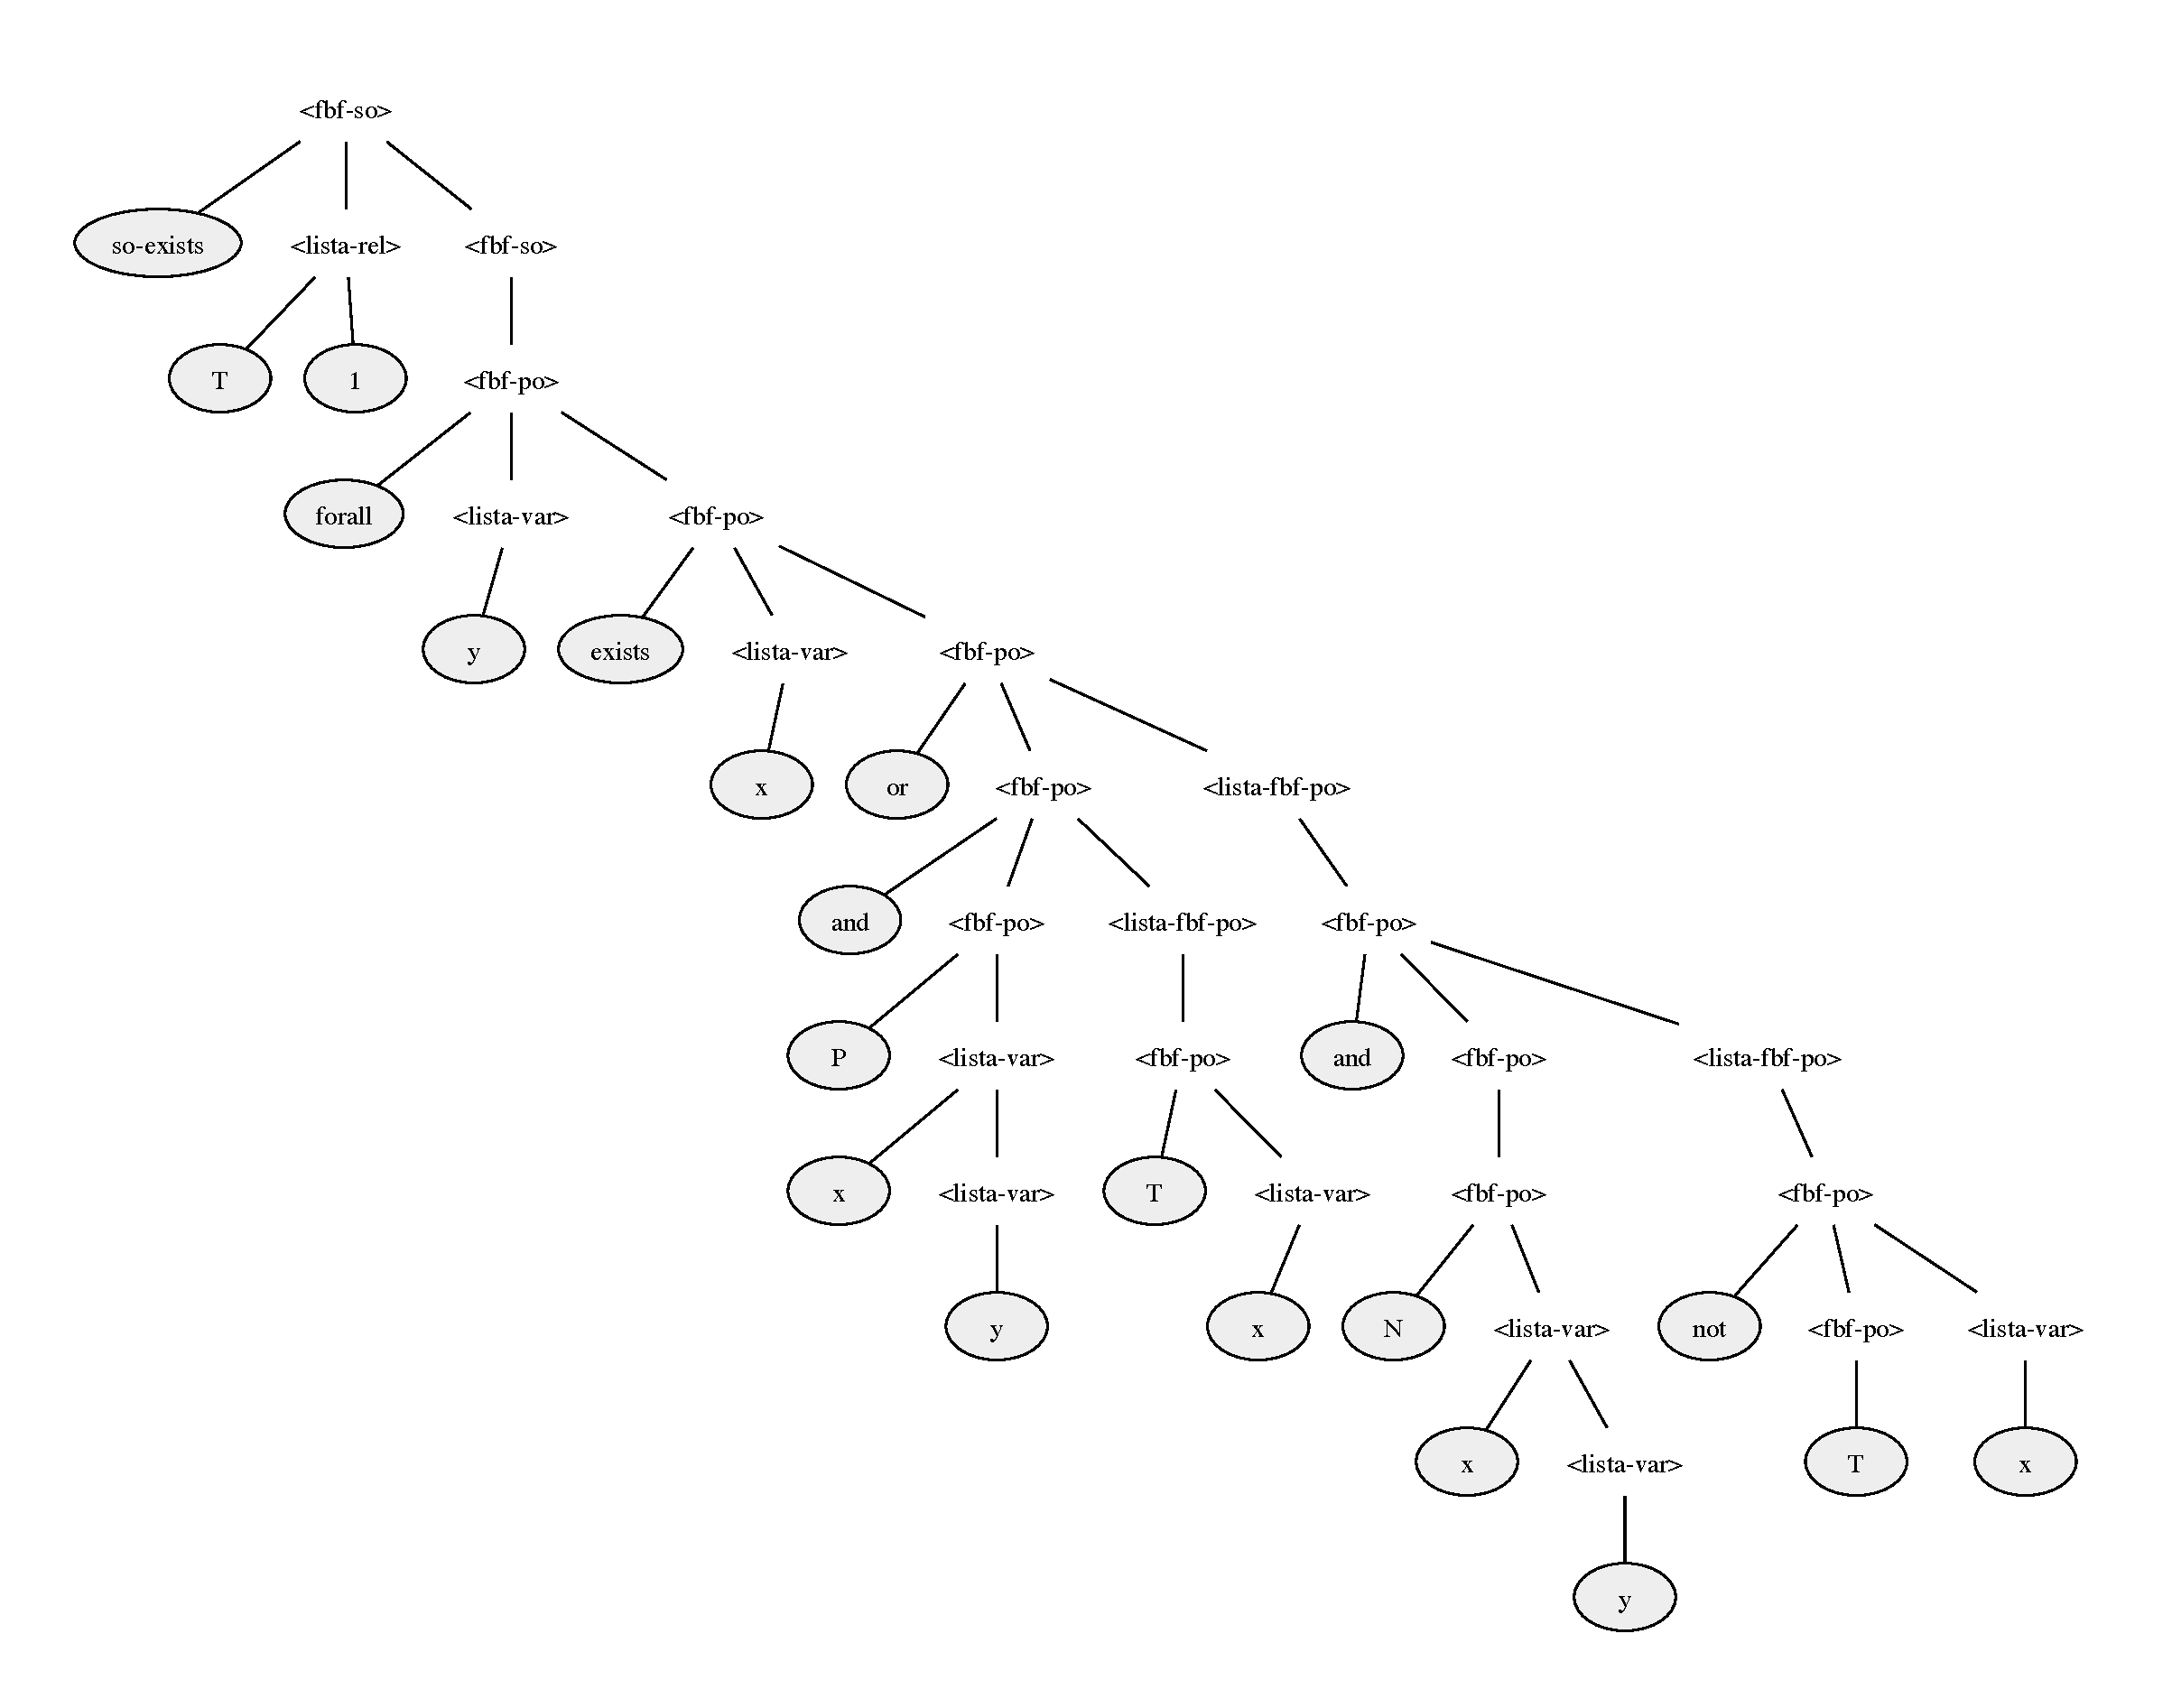
\includegraphics[width=\textwidth]{figuras/arbolsintaxis.pdf}
\caption{Árbol sintáctico que construye el \textit{parser} al analizar la
sentencia $\Phi_{SAT}$. Los nodos terminales se marcan con un óvalo.}
\label{esquema_herramienta}
\end{figure}
\end{landscape}
